%%%%%%%%%%%%%%%%%%%%%%%%%%%%%%%%%%%%%%%%%%%%%%%%%%%%%%%%%%%%%%%%%
\chapter{EXPERIMENTS}\label{ch:CH5}
%%%%%%%%%%%%%%%%%%%%%%%%%%%%%%%%%%%%%%%%%%%%%%%%%%%%%%%%%%%%%%%%%

All the code used for the experiments explained in this chapter can be found on master branch of the GitHub public repository: \newline \hyperrefurl{https://github.com/ozanguldali/modelsWithLASSO}. 

Python programming language in version of 3.7.6 combining with Clang 4.0.1 was used to train, test and classify on our environment. PyTorch module with the torch version of 1.5.0, the torchsummary version of 1.5.1 and the torchvision version of 0.6.0, and Scikit-learn library with the version of 0.23.2 were used for CNN and ML coding respectively. All experiments were performed on the Google Colaboratory using its GPU with the number of workers as four.

\section{Dataset}

The basis data was obtained from GitHub platform repository which can be reached via link \hyperrefurl{https://github.com/ieee8023/covid-chestxray-dataset/}. On the GitHub repository, the data are placed in \href{https://github.com/ieee8023/covid-chestxray-dataset/tree/master/images}{"images"} folder and the information file about data is in \href{https://github.com/ieee8023/covid-chestxray-dataset/blob/master/metadata.csv}{'metadata.csv'} file.

To constuct the dataset, the metedata.csv file was parsed and data were filtered depending on whether it has age and sex info or not, the its finding includes "COVID-19" term or not, its modality is "X-ray" or not, and its view is "PA" or not. First, data having sex and age info, modality as "X-ray", and view as "PA" were chosen. Then two main classes were constructed by separating the chosen data whether its finding includes "COVID-19" or not. The data including "COVID-19" in its finding were labeled as "COVID-19" and the others were labeled as "non-COVID-19". Finally, in the ratio of 0.8, the labeled data were divided into train and test sets. At the end, 131 "COVID-19" and 123 "non-COVID-19" labeled data were obtained and splitted into train and test sets. Train set includes 105 "COVID-19" and 98 "non-COVID-19" labeled data, while test set includes 26 "COVID-19" and 25 "non-COVID-19".

\begin{figure}[h]
	\centering
	\subfigure[Train COVID-19 Data]{\label{fig:dataset_samples_a}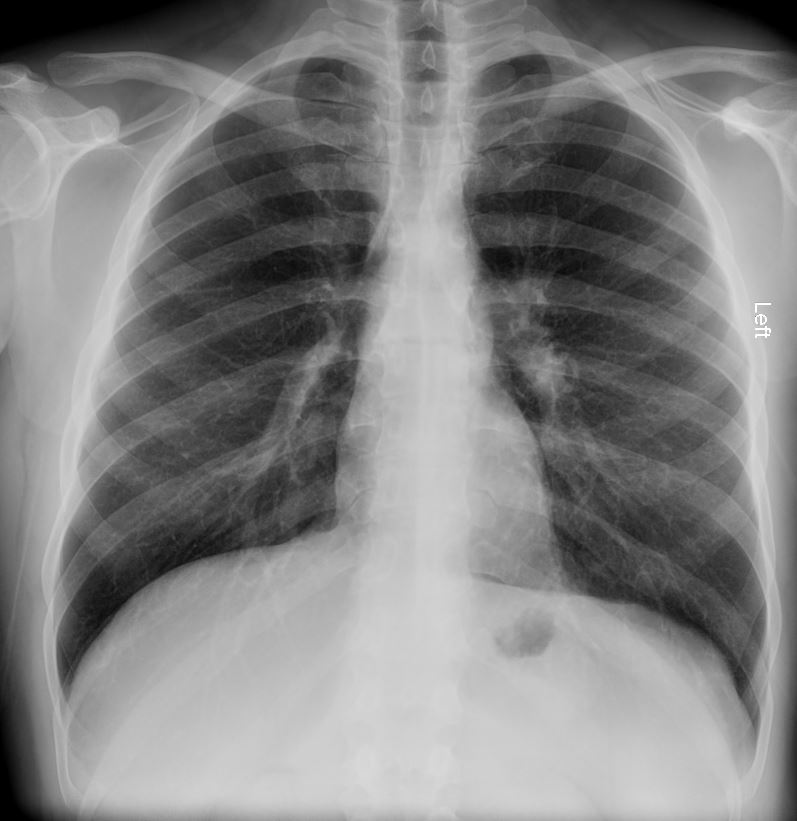
\includegraphics[width=.4\linewidth,height=.4\linewidth,scale=0.6]{fig/train_covid_data.jpg}}
	\subfigure[Test non-COVID-19 Data]{\label{fig:dataset_samples_b}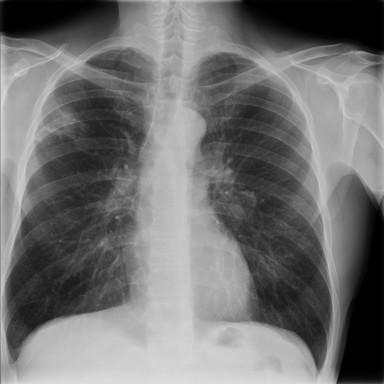
\includegraphics[width=.4\linewidth,height=.4\linewidth,scale=0.6]{fig/test_non_covid_data.jpg}}
	\caption{Dataset Samples.}
	\label{dataset_samples}
\end{figure}

Data are appeared in different formats such that .png, .jpg, .jpeg, in different aspect rations and dimensions such as 384×384, 462×450, etc, and in different sizes such as 606 KB, 69 KB, 1 KB, etc. Thus, before using the data, each datum was resized to 224x224, center cropped, gray scaled and normalized by the mean of (0.485, 0.456, 0.406) and the standard deviation of (0.229, 0.224, 0.225) for red, blue and green channels respectively.

\begin{figure}[h]
	\centering
	\subfigure[Original (826×768)]{\label{fig:data_transform_steps_a}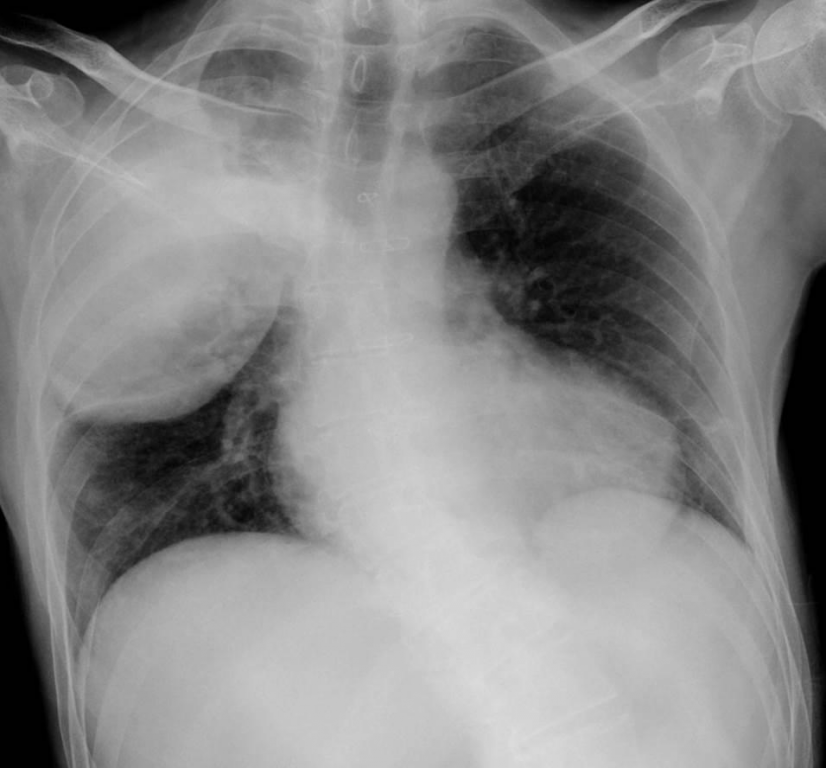
\includegraphics[width=.35\linewidth]{fig/test_covid_data.jpg}}
	\subfigure[Resized, Square Cropped and Gray-Scaled]{\label{fig:data_transform_steps_b}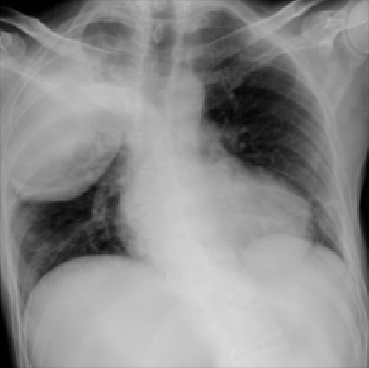
\includegraphics[width=.25\linewidth]{fig/test_covid_data_cropped.png}}
	\subfigure[Normalized]{\label{fig:data_transform_steps_c}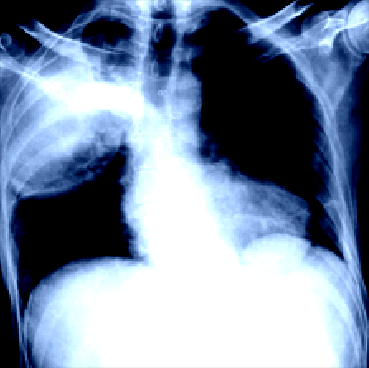
\includegraphics[width=.25\linewidth]{fig/test_covid_data_cropped_normalized.png}}
	\caption{Image Transformation Steps - Test COVID-19 Sample.}
	\label{data_transform_steps}
\end{figure}

\section{Data Augmentation}

While data sizes on classes are unbalanced, one or more data augmentation techniques are used on train data to balance them. Furthermore, for a balanced dataset, one can use data augmentation to increase the train data size.

Data augmentation techniques on visual data can be classified in 2 groups such that position augmentation and color augmentation. Position augmentation takes the original data and applies the desired operations from followings: flipping, rotation, translation and scaling. On the other hand, during the color augmentation, the augmented datum is obtained by changing one or more of followings: hue, saturation, brightness and contrast. If n kind augmentation choice is used to m number of data, at the end m*(n+1) data are obtained. That is the summation of n augmented datum for each sample of m data, and the original m samples.

In the thesis, position augmentation with horizontal flip, vertical flip, 90 degrees of rotation, 180 degrees of rotation and 270 degrees of rotation is used on the whole train data. These augmented data are not physical, i.e. not saved as files, and only used on CNN training process. Data augmentation is not used on ML processes.

The number of data on train and test sets for each class after augmentation can be seen on Table~\ref{tab:final_dataset_size}.


\begin{table*}[h]
{
    \setlength{\tabcolsep}{14pt}
    \caption{The detailed number of data.}
    \begin{center}
    % \vspace{-6mm}
    \begin{tabular}{lccrrrrr}
    \hline\hline
    \multirow{2}{*}{\textbf{Class}} & \multirow{2}{*}{\textbf{Original Set}} & \multicolumn{2}{c}{\textbf{Train Set}} & \multirow{2}{*}{\textbf{Test Set}} \\ \cline{3-4}
                           &                               & \textbf{Chosen}  & \textbf{After Augmentation}  &    \\
    \hline
    COVID-19           & 131                           & 105     & \multicolumn{1}{c}{630} & \multicolumn{1}{c}{26} \\
    non-COVID-19               & 123                           & 98      & \multicolumn{1}{c}{588} & \multicolumn{1}{c}{25} \\
    TOTAL                  & 254                           & 203     & \multicolumn{1}{c}{1218} & \multicolumn{1}{c}{51} \\   
    \hline
    \end{tabular}
    % \vspace{-6mm}
    \end{center}
    \label{tab:final_dataset_size}
}
\end{table*}

\begin{figure}[h]
	\centering
	\subfigure[Original Sample - Train non-COVID-19]{\label{fig:augmented_sample_a}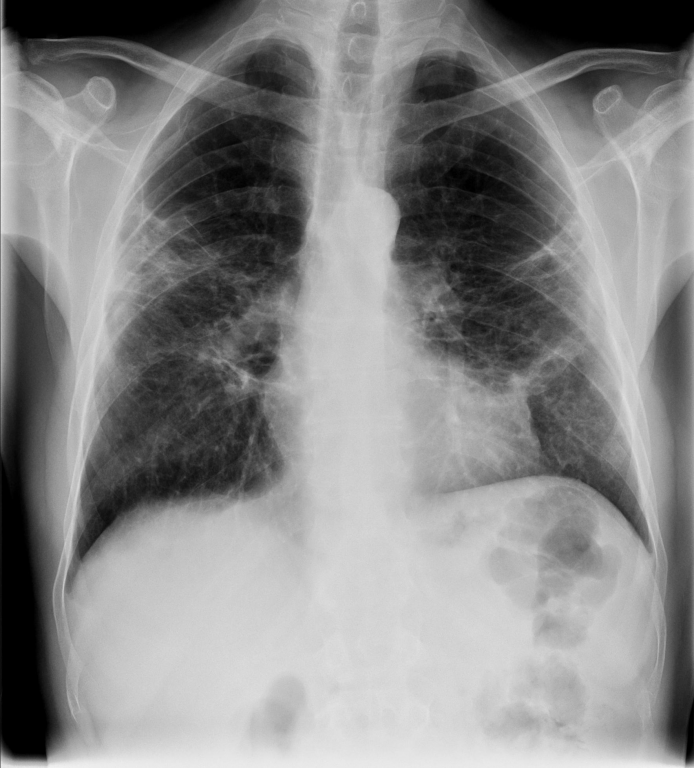
\includegraphics[width=.3\linewidth]{fig/train_non_covid_data.jpg}}
	\subfigure[Horizontal Flipped]{\label{fig:augmented_sample_b}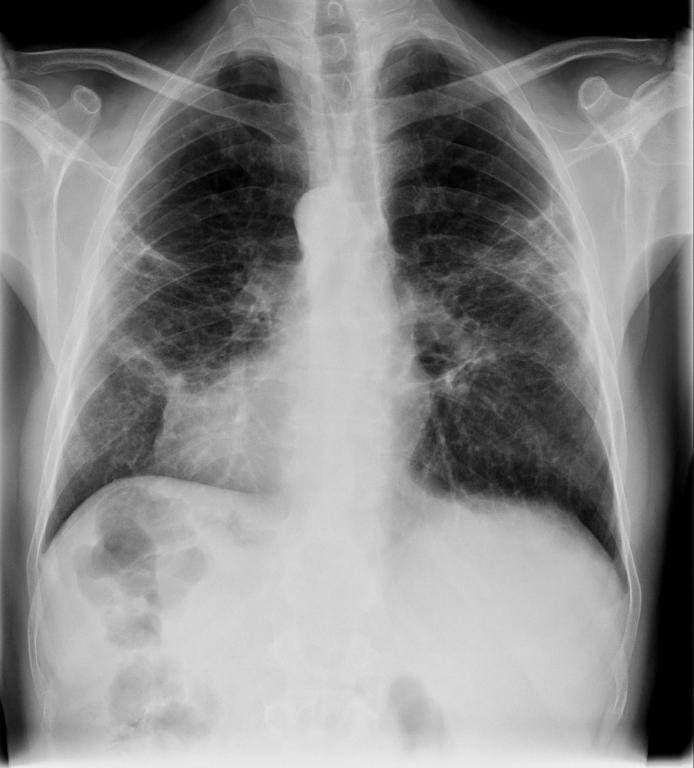
\includegraphics[width=.3\linewidth]{fig/horizontalFlipped_train_non_covid_train_data.jpg}}
	\subfigure[Horizontal Flipped]{\label{fig:augmented_sample_c}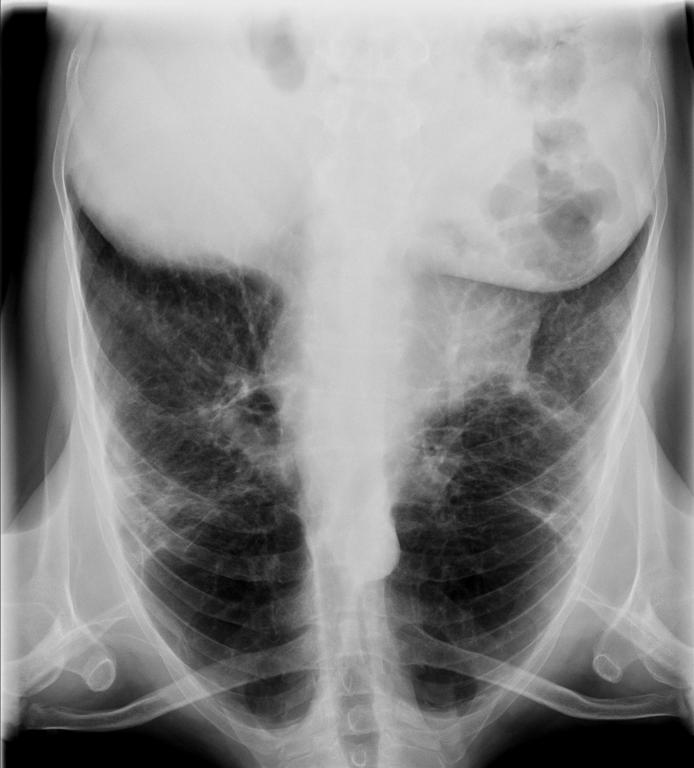
\includegraphics[width=.3\linewidth]{fig/verticalFlipped_train_non_covid_train_data.jpg}}
	\subfigure[Horizontal Flipped]{\label{fig:augmented_sample_d}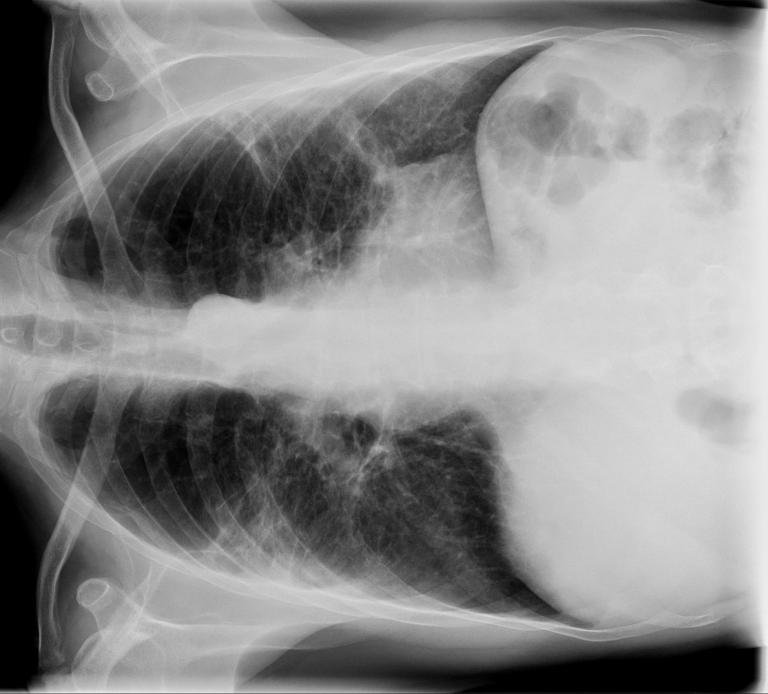
\includegraphics[width=.3\linewidth]{fig/90Rotated_train_non_covid_train_data.jpg}}
	\subfigure[Horizontal Flipped]{\label{fig:augmented_sample_e}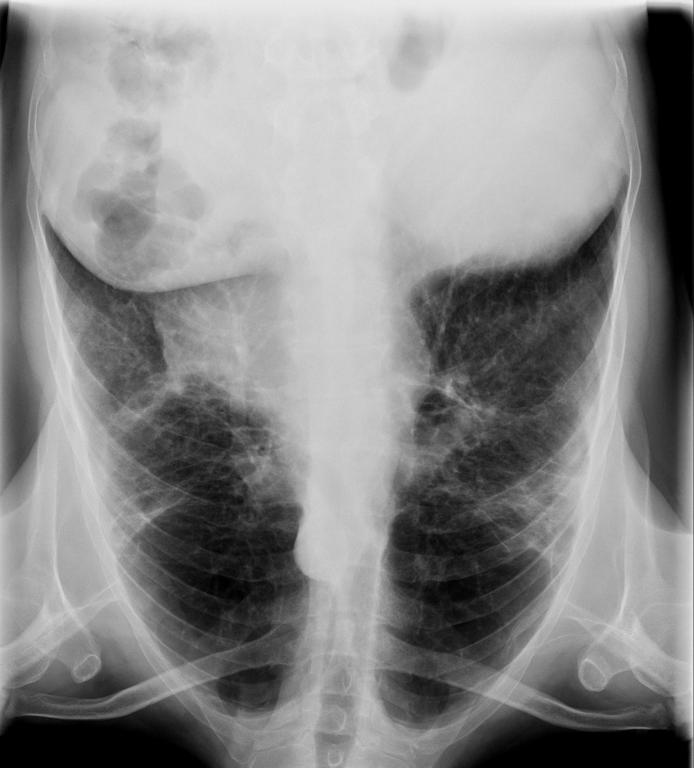
\includegraphics[width=.3\linewidth]{fig/180Rotated_train_non_covid_train_data.jpg}}
	\subfigure[Horizontal Flipped]{\label{fig:augmented_sample_f}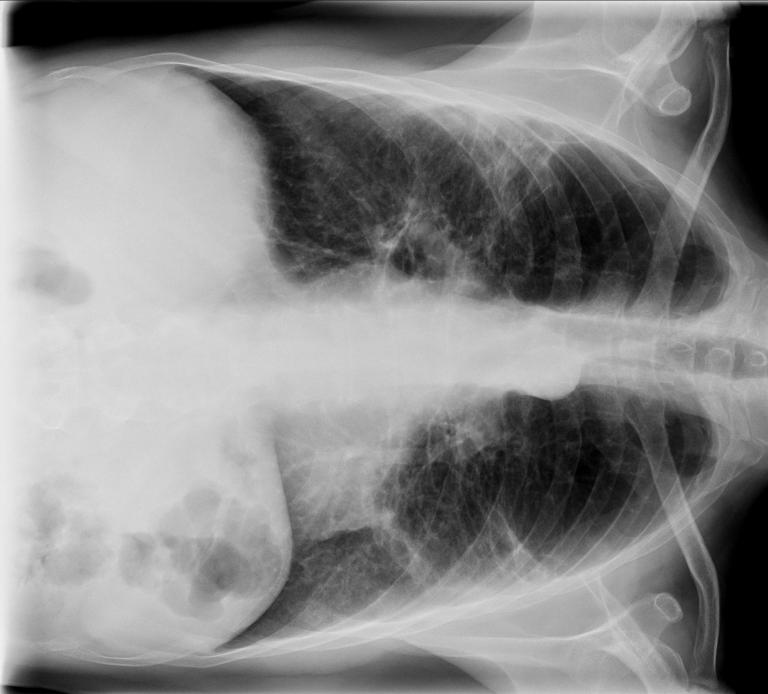
\includegraphics[width=.3\linewidth]{fig/270Rotated_train_non_covid_train_data.jpg}}
	\caption{Original Sample and Augmentation.}
	\label{augmented_sample}
\end{figure}

\section{Training and Testing on Convolutional Neural Network Models}\label{sec:CH5_cnn_experiments}

All CNN experiments was made on pre-trained CNN models. That is, the corresponding model weights was used with different strategies to feed the models.

Since our dataset is obviously small and the data content is different from ImageNet dataset \cite{imagenet}, we experimented to train the entire model, and to freeze the first few layers and train others. The frozen layers for each experiment model are:

\begin{itemize}
    \item the first convolution layer, and its following ReLU and maximum pooling layers for AlexNet architecture,
    \item the first convolution layer, and its following batch normalization, ReLU and maximum pooling layers for ResNet architectures, and
    \item the first six layers which are in order of convolution, batch normalization, ReLU, convolution, batch normalization, ReLU and maximum pooling layers for VGG architectures.
\end{itemize}

The comparison results have shown that, training the entire model instead of freezing the stated number of layers above gives more minimal losses and more accurate classification results. However, it must be remarked that, even the number of frozen layers are not much, since the number of parameters are less on this technique than entire model training, the computation time of each batch is observably shorter as well. 

Train data were set to be shuffled on each epoch and the batch size was experimentally set from $2^4$ to $2^6$. The number of epoch was set to 50, and the validation period was set as $1/50$. That is, before the first training epoch and after each training epoch, validation process was applied on test set. On each validation, the saved model weights files for corresponding configurations were checked. If there exists no saved file having greater accuracy percentage than the current state, the current model weights are saved as a new model weight *.pth file with the name including the validation result and training configurations. The saved CNN model weights files can be found under the \textit{/cnn/saved\_models} directory of project repository at \hyperrefurl{https://github.com/ozanguldali/modelsWithLASSO}. After the last training epoch, test process is applied rather than validation, and the same accuracy comparison over saved *.pth files is executed. That is why, the number of validation accuracy results are 50 whereas the number of validation losses are 49. The reason why we limited the epoch size as 50 is that, the models were overfitting after this number, and even before sometimes.

By our weights file comparison rule, there may be multiple *.pth weights files for the same configuration and accuracy value. This time, the train loss values, before the validation or test result obtained, and the validation loss values, if available, are considered. Here, the less loss is better to choose.

The cross-entropy loss function, explained in Section~\ref{sec:CH3_cross_entropy}, was used for all CNN models. To optimize it, Adam, SGD Momentum and Adam with decoupled weight decay optimizers were experimented with various learning rate, momentum and weight decay parameter values. Moreover, the learning rate was experimentally scheduled by the reducing rate as 0.1 for each quarter of total epoch size. However, the scheduler approach drove the models to overfitting. 

Final hyper-parameters experienced as the best for each model and each optimizer differ. The best ones for ResNet-50 model can be seen in Table~\ref{tab:cnn_hyperparameters}. Furthermore, on our experiments, we encountered the optimal batch size, in terms of computational time and obtained losses, as $2^4$. Hence, the number of iteration on each epoch was 77 for augmented train data, and 4 for test data which was used on both test and validation processes.

\begin{table}[h]
\centering
\caption{CNN models final hyper-parameters.}
\label{tab:cnn_hyperparameters}
\begin{tabular}{lccc}
\multicolumn{1}{c}{\textbf{Optimizer}} & \textbf{Learning Rate} & \textbf{Momentum} & \textbf{Weight Decay} \\
SGD Momentum                           & 1e-4                   & 0.9               & -                     \\
Adam                                   & 1e-5                   & -                 & 1e-3                     \\
AdamW                                  & 1e-5                   & -                 & 1e-4                 
\end{tabular}
\end{table}

All pre-trained CNN models were experimented by setting the final layer out feature size as the class size, i.e. 2. Furthermore, for all architectures experienced in this thesis, a modification is applied on the classification section as adding a block of ReLU, dropout and fully-connected layers in order after the last fully-connected layer.

For ResNet-50 model, the total parameters, so the total trainable parameters on full-training, is 25,559,034 for one sample. For an input image in the size of 0.59 MB, forward and backward pass size is 309.48 MB and parameters size is 97.50 MB. Hence, the estimated total size of one iteration on this image is 407.57 MB according to PyTorch.

\begin{landscape}
\begin{figure}[h]
    \centering
    \includegraphics[width=\linewidth]{fig/resnet50_visualization.png}
    \vspace{1mm}
    \caption{The sample visualization representing one iteration on ResNet-50 architecture and class probability result for COVID-19 labeled data from our dataset. The higher resolution version of image is available at \\  \hyperrefurl{https://github.com/ozanguldali/modelsWithLASSO/blob/master/figures/resnet50_visual.png}}
    \label{fig:resnet50_visualization}
\end{figure}
\end{landscape}

The higher resolution version of images in Figure \ref{fig:resnet50_visualization}, such as the visualizations of convolution blocks, is available at directory \hyperrefurl{https://github.com/ozanguldali/modelsWithLASSO/blob/master/figures}.

\section{Deep Feature Extraction}

After training, validating and testing the dataset on pre-trained CNN models, the deep feature extraction progress was started. Since the best results according to accuracy are stored, these model weights files are used to extract deep features from their corresponding CNN architectures.

Here, the modifications on CNN models stated at previous section show its another purpose. The deep feature are extracted from these added or replaced fully-connected layers as:

\begin{itemize}
    \item using the third fully-connected layer for AlexNet architecture,
    \item using the first fully-connected layer for ResNet architectures, and
    \item using the third fully-connected layer for VGG architectures.
\end{itemize}

The deep features extracted from CNN models are used to feed machine learning algorithms to improve the classification success.

\begin{figure}[h]
    \centering
    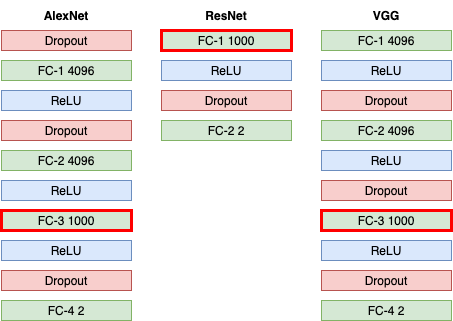
\includegraphics[width=.8\linewidth]{fig/modified_classification_blocks.png}
    \vspace{2mm}
    \caption{Modified classification blocks where bold red windowed fully-connected layers denotes the deep feature extraction state.}
    \label{fig:modified_classification_blocks}
\end{figure}

\section{Forming the Feature Maps} \label{sec:CH5_forming_features}

In this study, we have two types of feature matrices and one consisting of their conjunction. The first feature matrix includes the deep features extracted by the help of CNN models. Instead of image segmentation, Red-Green-Blue (RGB) color codes or manual image partition labeling, we use the features derived from deep learning process. The number of features are 1000 for each CNN architecture, because of the output size of used fully-connected layers. We denote the matrix of deep features as $X_{cnn}$ and the feature size as $d_{cnn} = 1000$.

On the other part, we have demographic information for each sample, and that is the why our dataset is restricted. We denote the matrix of demographic information as $X_{info}$ and the feature size as $d_{info} = 2$. Age information was categorized to 5 groups such as under 18, between 18 and 37, between 39 and 59, between 60 and 79, and over 80 ages.

Hence, the merged features matrix denoted by $X_{all}$ has the feature size as $d_{all} = 1002$.

\begin{figure}[h]
    \centering
    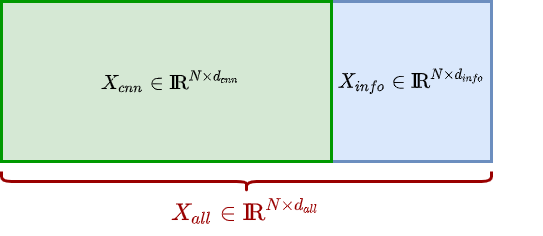
\includegraphics[width=.6\linewidth]{fig/feature_maps.png}
    \vspace{2mm}
    \caption{Feature maps where $d_{cnn} = 1000$, $d_{info} = 2$, and $d_{all} = d_{cnn} + d_{info} = 1002$.}
    \label{fig:feature_maps}
\end{figure}

\section{Data Pre-Processing}

\subsection{Data Standardization}

Machine learning estimators commonly requires data standardization; because, the data may not be always in the form of standard normal distribution. There are three basic ways to standardize the data such as 1) centering data with the mean, 2) scaling data with the standard deviation, and 3) centering and scaling data with the main and standard deviation. In the experiments, we only centered the data. That is, we set $\mu$ as the mean of training samples and $\sigma$ as 1 in the equation (\ref{eq:data_standardization}):

\be
\label{eq:data_standardization}
Z = (X - \mu * I) / \sigma\:.
\ee

\subsection{Data Normalization}

Data normalization scales each individual sample to have a unit norm in the rational numbers range [0.0, 1.0]. Two ways of normalization was experimented which are least absolute technique, known as L1 normalization, and least squares technique, known as L2 normalization.

\begin{itemize}
    \item \textbf{L1 Norm:} Scales the sum of the absolute differences of each individual feature on a sample to 1. That is, scales the $S_{L1}$ to 1 in the equation (\ref{eq:data_l1_norm}):
    
    \be
    \label{eq:data_l1_norm}
    S_{L1} = \sum_{i=1}^{d} \big|y_{k} - X_{k,i}\big|\:,
    \ee
    
    where d is the number of features, $X_{k}$ is the $k^{th}$ sample and $X_{k,i}$ is the $i^{th}$ feature value of corresponding sample, and $y_{k}$ is the target value for corresponding sample. Here, the scaling ratio is $1 / S_{L1}$; thus, $X_{k} / S_{L1}$ gives the L1 normalized feature values for this sample.
    
    \item \textbf{L2 Norm:} Scales the sum of the squares of differences of each individual feature on a sample to 1. That is, scales the $S_{L2}$ to 1 in the equation (\ref{eq:data_l2_norm}):
    
    \be
    \label{eq:data_l2_norm}
    S_{L2} = \sum_{i=1}^{d} \big(y_{k} - X_{k,i}\big)^{2}\:,
    \ee
    
    where d is the number of features, $X_{k}$ is the $k^{th}$ sample and $X_{k,i}$ is the $i^{th}$ feature value of corresponding sample, and $y_{k}$ is the target value for corresponding sample. Here, the scaling ratio is $\sqrt{1 / S_{L2}}$; thus, $X_{k} / \sqrt{S_{L2}}$ gives the L2 normalized feature values for this sample.
\end{itemize}

We used the L2 normalization as the final settings of the data pre-processing pipeline.

\section{Hyper-Parameter Tuning}

For each machine learning algorithm, there exists several hyper-parameters. Since the hyper-parameter settings cannot be generalized, and so differ for each problem and dataset, finding the optimal combination of hyper-parameters is a separate mission. Which characteristic to look for when choosing the most optimal hyper-parameter combination depends on the problem and the researcher. In this thesis, we decide according to accuracy values. There are three common optimization method such that bayesian optimization, grid search and random search.

\begin{itemize}
    
    \item \textbf{Grid Search:} all combinations between hyper-parameter options are experimented. For instance, if there exists $m$ number of hyper-parameters and each of them has $a_{i}$ options where $a_{i}$'s are positive integers for $i \in \{1,2,\dots,m\}$, then the total number of grid search iterations are $\prod_{i=0}^{m} a_{i}$. Moreover, if K-Fold cross validation is applied, the number of iterations are raised to $K \times \prod_{i=0}^{m} a_{i}$.
    
    \item \textbf{Random Search:} randomly chosen hyper-parameter option combinations over all are experienced. The number of combinations to be tried are determined by researcher as less than the total number of combinations.
    
    \item \textbf{Bayesian Optimization:} this methodology is based on Bayesian Principle. While the combinations of hyper-parameter options are experimented, the previously known results leads to create a new combination space by using bayesian rule. This time, the choice of combinations are not random, but depend on the useful or irrelevant combination estimation.
    
\end{itemize}

In thesis, we experimented grid search with 10-Fold cross validation.

\section{Training and Testing on Machine Learning Models}

The partitioning of dataset into train and test sets are preserved on machine learning stage. The only difference is, data augmentation is not applied on train set. 

All three types of feature matrices were experienced separately. For each, 10-Fold cross validation was applied on train set only by using grid search to find the generalized optimal combination of hyper-parameter options. To decide the best combination, the first criterion was set as accuracy value, and if there exists multiple same values, the second criterion was determined as the computation time. If there exists combinations such that two of criteria are the same, the last experienced combination was chosen. 

For the repeatability of our work, we initialized the Python random number generation with different seeds. In other words, the seed parameter of Python random library is one of out hyper-parameters, and we chose the best seed among our experiments to achieve final results.

Here, a parenthesis must be open for linear discriminant analysis algorithm. Since there is no library in Python that supports regularization on LDA, we used TULIP package \cite{TULIP_package} on version 1.0.1 in R programming language with the version of 4.0.3 to implement L1 regularized LDA model. Furthermore, grid search tuning was not applied to this model. Hyper-parameter tuning process was applied only for seed and regularization parameters.

Penalty terms, which are no penalty, Lasso and Ridge, were not considered as hyper-parameters, because they were experienced and compared separately. All hyper-parameter options to be combined can be found in Tables~\ref{tab:svm_hyperparameter_table} -~\ref{tab:lda_hyperparameter_table}.

\begin{table}[h]
\centering
\caption{SVM algorithm hyper-parameters to tune.}
\label{tab:svm_hyperparameter_table}
\begin{tabular}{lcc}
\multicolumn{1}{c}{\textbf{Hyper-Parameter}} & \textbf{Ridge Penalty}            & \textbf{Lasso Penalty} \\ \hline \hline
Kernel Function                              & linear, sigmoid, rbf     & linear               \\ \hline
Regularization Parameter                     & \begin{tabular}[c]{@{}c@{}}5e-5, 1e-4, 2e-4, \\ 5e-4, 5e-3, 1e-2, \\ 2e-2, 5e-2, 0.1, \\ 0.5, 1.0, 2.0, \\ 5.0, 10.0, 15.0\end{tabular}                        & \begin{tabular}[c]{@{}c@{}}5e-5, 1e-4, 2e-4, \\ 5e-4, 5e-3, 1e-2, \\ 2e-2, 5e-2, 0.1, \\ 0.5, 1.0, 2.0, \\ 5.0, 10.0, 15.0\end{tabular} \\ \hline           
\end{tabular}
\end{table}

\begin{table}[h]
\centering
\caption{LR algorithm hyper-parameters to tune.}
\label{tab:lr_hyperparameter_table}
\begin{tabular}{lccc}
\multicolumn{1}{c}{\textbf{Hyper-Parameter}} & \textbf{No Penalty}                                                    & \textbf{Lasso Penalty}                                                    & \textbf{Ridge Penalty}                                                            \\ \hline \hline
Solver Function                              & \begin{tabular}[c]{@{}c@{}}newton-cg, lbfgs, \\ sag, saga\end{tabular} & liblinear, saga                                                           & \begin{tabular}[c]{@{}c@{}}newton-cg, lbfgs, sag, \\ saga, liblinear\end{tabular} \\ \hline
Regularization Parameter                     & -                                                                      & \begin{tabular}[c]{@{}c@{}}5e-5, 1e-4, 2e-4, \\ 5e-4, 5e-3, 1e-2, \\ 2e-2, 5e-2, 0.1, \\ 0.5, 1.0, 2.0, \\ 5.0, 10.0, 15.0\end{tabular} & \begin{tabular}[c]{@{}c@{}}5e-5, 1e-4, 2e-4, \\ 5e-4, 5e-3, 1e-2, \\ 2e-2, 5e-2, 0.1, \\ 0.5, 1.0, 2.0, \\ 5.0, 10.0, 15.0\end{tabular}         \\ \hline
\end{tabular}
\end{table}

\begin{table}[h]
\centering
\caption{KNN algorithm hyper-parameters to tune.}
\label{tab:knn_hyperparameter_table}
\begin{tabular}{lc}
\multicolumn{1}{c}{\textbf{Hyper-Parameter}} & \textbf{No Penalty}                                 \\ \hline \hline
Number of Neighbors                          & 3, 5, $\sqrt \text{the number of samples}$                         \\ \hline
Type of Majority Voting                      & uniform, weighted                                   \\ \hline
Neighborhood Finder                          & \multicolumn{1}{l}{brute force, ball tree, k dimensional tree} \\ \hline
Metric Function                              & \multicolumn{1}{l}{euclidean, manhattan, chebyshev} \\ \hline
\end{tabular}
\end{table}

\begin{table}[h]
\centering
\caption{LDA algorithm hyper-parameters to tune.}
\label{tab:lda_hyperparameter_table}
\begin{tabular}{lcc}
\multicolumn{1}{c}{\textbf{Hyper-Parameter}}                                                                 & \textbf{No Penalty} & \textbf{Lasso Penalty}                                                   \\ \hline \hline
Regularization Parameter                                                                                     & -                   & \begin{tabular}[c]{@{}c@{}}5e-5, 1e-4, 2e-4, \\ 5e-4, 5e-3, 1e-2, \\ 2e-2, 5e-2, 0.1, \\ 0.5, 1.0, 2.0, \\ 5.0, 10.0, 15.0\end{tabular} \\ \hline
Solver Function                                                                                              & svd, lsqr, eigen    & -                                                                        \\ \hline
\begin{tabular}[c]{@{}l@{}}Computing the Weighted \\ Within-Class Covariance\\ (for svd solver)\end{tabular} & Yes, No             & -                                                                        \\ \hline
\end{tabular}
\end{table}

When the optimal hyper-parameter combination was determined with the aim of generalization, the model weights obtained by training on corresponding machine learning algorithm with these hyper-parameters are used on testing stage. The final results are achieved by testing on this fitted model. Furthermore, another grid search was applied on determined train and test data, and the results were compared by the generalized ones.